\documentclass[12pt, English]{article}
\usepackage[utf8]{inputenc}
\usepackage[top=1in, bottom=1in, left=1in, right=1in]{geometry}
\usepackage{setspace}
\usepackage{adjustbox}
\usepackage{graphicx}
\usepackage{amsmath}
\usepackage{indentfirst}
\usepackage{graphicx}
\usepackage{natbib}
\usepackage{booktabs}
\usepackage{flafter}
\usepackage{csquotes}
\usepackage{rotating}


\title{Influence of Gubernatorial Elections on the Gender Wage Gap}
\author{Abigail Hoffman}
\date{December 17, 2021}


\begin{document}
\maketitle
\begin{abstract}

This paper uses a fixed effects regression model to analyze the influence of gubernatorial election results on the gender wage gap in the United States of America from 1994 through 2018. Fixed effects modeling methods applied to sets of group means in cases when certain groups are exposed to the causing variable of interest and others are not. I have hypothesized that when the democratic gubernatorial election holds a majority of voter percentages, the gender wage gap will decrease. 
\end{abstract}

\newpage

\section{Introduction}
\doublespacing
\subsection*{History of the Woman Suffrage Movement}
During the mid-nineteenth century, the fight for women's suffrage in the United States began. Despite a wide variety of oppressive policies being identified by the suffrage group, the right to vote was the spark that ignited the movement. The initial declaration of the movements intention was encompassed within the Declaration of Sentiments written by Elizabeth Cady Stanton in 1848, later signed by fellow members of the women's suffrage movement. This was a strategic parallel to the actions of the founding fathers. Stanton directly connected the emerging campaign for women's rights to a powerful American symbol of liberty, the Declaration of Independence. 
\begin{displayquote}

The opening began like its predecessor: "We hold these truths to be self-evident; that all men and women are created equal; that they are endowed by their Creator with certain inalienable rights; that among these are life, liberty, and the pursuit of happiness. Elizabeth Cady Stanton's draft continued: Now, in view of this entire disenfranchisement of one-half the people of this country, their social and religious degradation, — in view of the unjust laws above mentioned, and because women do feel themselves aggrieved, oppressed, and fraudulently deprived of their most sacred rights, we insist that they have immediate admission to all the rights and privileges which belong to them as citizens of these United States" \citep{NWHA}.
\end{displayquote}

Several Activists continued their mission to secure women's right to vote despite the initial backlash and ridicule that derived from the publication of the Declaration of Sentiments. Their work continued into the early twentieth century as the campaign for woman suffrage met such staunch opposition, it took 72 years for the women and their male supporters to be successful. Passed by Congress June 4, 1919, and ratified on August 18, 1920, the 19th amendment guarantees all American women the right to vote \citep{NINETEENTH}. 


\subsection*{Second Wave Feminism}
The fight for equity and equality continued into the 1960s, which sparked the second wave of the women's rights movement. This movement is also known as the second wave of feminism. In 1961, President Kennedy named Eleanor Roosevelt the chair of the Commission on the Status of Women to better understand a woman's role in American society.  In 1963, the Commission published a report that indicated that women experienced discrimination in almost every part of American life.  

After this revelation, the novel by Betty Friedan, The Feminine Mystique, documented the mental oppression that the limited role of homemaker could provide women. Despite having an education, women were still limited by the status of their male counterparts. Friedan surveyed women from her university reunion to use their experience as data to document and explain the universal melancholy of women from that era. The term melancholy is now commonly known as depression and is a mental illness. The novel proceeded to inspire thousands of women to look for fulfillment beyond the role of homemaker.

The second wave of feminism erupted like the tide, rippling effects long after emergence. Financial liberation emerged through these ripples. The movement enabled women to have a credit card in their own name and no longer required a male cosigner to finance a bank loan. The National Organization for Women (NOW) argued the issue of segregated female and male occupation ads to the Supreme Court. This stage of notoriety in the judicial system allowed for the shift in public perception of female roles. After the case adjourned, the Supreme Court ruled in favor of a woman to be able to hold a job for which she was qualified. 

Now, women can hold any occupation in previously considered male-dominated fields. As we can see by Figure 1, female labor participation dramatically increased through changes in the law and legislation along with support from politicians resulting in the course of action against discrimination by gender \citep{USBureauofLaborStatistics1}. Despite the ignited liberation for women, they were still not considered equal by pay. During this decade, it was noted that women were earning only a little over a half of their male coworkers pay. Moreover, for women of color earnings diminishes further. Equality in wages earned remains a persistent issue in today's culture and will continue disproportionately shaping the worldwide economy. 

\subsection*{Gender Wage Gap}
Although the gender wage gap is not a new economic problem in today's society, it is a persistent problem that continues to pay women less than their male counterparts disproportionately. Although legislation has continued to move forward for equality and equity based on gender, race, and sexual orientation, the problem remains. Female workers earn 80 to 82 cents on their male counterpart's dollar \citep{bureau_2021}. According to the U.S. Census Bureau, "women's human capital and labor force characteristics that drive wages increasingly resemble men's, so remaining differences in these characteristics explain less of the gender wage gap now than in the past" \cite{bureau_2021}. The gender pay gap is attributed to a plethora of factors, including occupational segregation, bias against working mothers, and direct pay discrimination. Additionally, such things as racial bias, disability, access to education, and age come into play \citep{AAUW}.

A visualization of the gender wage gap from the 1970s through 2021 is shown in Figure 2 in the Figures and Tables section \citep{USBureauofLaborStatistics2}. The data is derived from FRED economic data created by the Federal Reserve Bank of St. Louis. 

\subsection*{Implications on Economic Conditions}
Closing the gender wage gap is a crucial element that could improve the health of the national economy in the United States. Equitable income would increase national and state tax revenues which then can be utilized to allow public improvement investments in education, transportation, roads, and other expenditures to cultivate more positive societal living standards. 

I have chosen to research the implication of gender on wages earned across the United States from 1994 through 2018 using data from the Community Population Survey \citep{IPUMSUSA}. Additionally, I am curious to understand if gubernatorial state-level politics (governor elected political affiliation) impact gender wage gaps. Often, the democratic party has a more significant percentage of female voters than the republican party. To better understand potentially why this occurs, taking into account which party more effectively combats the gender wage gap could result in changes in the persistent pattern of political party voting in state-level gubernatorial elections. My target audience is fellow researchers seeking to understand better the gender wage gap and fellow women voters who want to understand better which of the two political party systems could diminish the gap. 


\newpage



\section{Literature Review}
Research into understanding the connection between political party influence on economic conditions for state level and national level politics has been over half a century in the making. Research synthesized within this literature review will date to the mid-1970s through 2021. To better understand how my research can add to the published literature, considerations are given to the following topics: short-run economic conditions on voter response, micro and macroeconomic effects on presidential voting preference, gubernatorial accountability for state economies, linear fixed effect regressions, and gender inequality with political party consideration. 

Research published in the 1970s utilizes economic conditions from the Great Depression to understand later voter responses within political parties. An initial understanding of the research considers the asymmetry of short-run economic impacts against long-term ones. According to Bloom and Price, "the effect of short-run economic conditions is reflected by greater voter concern over the economy and less favorable evaluation of the administration's performance relative to the economy" \citep{bloom1975voter}. A political party in office is punished heavier when economic times are bad than rewarded for good economic conditions. Bloom and Price's research concluded with the identification of the asymmetric version of Kramer's original model that indicates voters tend to reduce votes for the incumbent's political party during economic downturns \citep{bloom1975voter}. 

Drawing from voter perception, Markus explains that voters have a sense of when times are good and when times are bad, resulting in their voting preference in the next election series \citep{markus1988impact}. Markus furthers the research and thought produced by Bloom and Price and adds consideration of understanding whether voters are pocketbook voters or, instead, the voters are sociotropic voters. A pocketbook voter is considered a supporter for the incumbent or his party and varies directly with their financial well-being. The sociotropic voter bases their political judgments on the nation's economic health rather than personal well-being. Despite not identifying the specific type of voter, the research focuses on individual voting choices in a linear regression model. The text utilizes a logit and probit model with instrumental variables. The research identified that "each 1 percent real increase in per capita disposable personal income increases the probability of incumbent vote by .023 (+.oo4)" \citep{markus1988impact}. Given that increased disposable income resulted in a better probability, there is a consideration that a specific political party is tied to decreasing the gender wage gap resulting in greater disposable income for women in society. 

Research by Niemi, Stanley, and Vogel uses the national economy condition to understand the impact on voter choice in gubernatorial elections \citep{niemi1995state}. The democratic party's embrace of female representation tends to shift to more liberal gender-related policies, resulting in this potential influence in better economic conditions rather than specific policy set in place by governors. Their research produces the opposite expected indication of party preference given that there is no significant impact with identified economic condition as not a crucial element for gubernatorial election results. 

According to Kuk and Hajnal, governors have a diminished ability to influence legislation \citep{kuk2021democratic}. Their model considers the economic conditions of inequality, like the gender wage gap, by using a Difference in Difference model. The result also indicated no significant levels of policy influence with democratic governors in office as opposed to republican governors in office \citep{kuk2021democratic}. 

\subsection*{Fixed Effect Model Consideration}
For this research project, the goal is to understand if gubernatorial voting margins by political parties reduce the gender wage gap. Previous research has indicated that linear regression models are used along with voter margin results to understand the type of voter and the economic impact on the nation economic well-being and personal pocketbooks. Literature has indicated that "fixed effects models are a primary workhorse for causal inference... used to adjust for unobservables in observational studies" \citep{imai2012use}. When implementing a fixed-effects model, the goal is to reduce selection bias in the model. In turn, this will reduce omitted variable bias, which would lead to a violation of a Gauss-Markov assumption if omitted variable bias arose in the model \citep{mummolo2018improving}. Utilizing a fixed-effects model into the research could build upon previous literature models to add further research on economic conditions with political party consideration.



\newpage
\section{Data}
\subsection*{Source of data}
I extracted my data from IPUMS-USA using sampling from the Community Population Survey (CPS). This data is verified and authorized by the Minnesota Population Center with an affiliation to the University of Minnesota. The Public Use Micro-data Set from the Community Population Survey uses data from the U.S. Census to easily identify critical variables and manipulate data for research purposes \citep{IPUMSUSA}. Data extracted focuses on 1994 through 2018 across the fifty United States, excluding the District of Columbia. The exclusion of District of Columbia is primarily due to the function of their mayor serving as a governor role rather than separate elections as the other fifty states have for state government checks and balances purposes. 

I used an additional data set found on the online source Kaggle. Kaggle is a subsidiary of Google LLC. It is an online community of data scientists and machine learning practitioners. Kaggle allows users to access and utilize data sets, explore and build models in a web-based data-science environment which adds to the collaborative efforts of open source data science. I utilized a data set that had collected data from 1972-2019 on Gubernatorial Election results made by \citep{KAGGLE}. The data was already standardized and allowed for easy statistical manipulation. I chose a random sample to verify the information was accurate. 

I set wages greater than 1 dollar to filter data representative of employed workers. I dropped values that returned not applicable (N/A) in any of the variables. My audience is targeted towards groups working to close the wage gap between marginalized groups and their white male counterpart. Understanding governor and presidential election party results will better inform voters for future legislative purposes.  

\subsection*{Description of Selected Variables}

The explained variable of wage was mutated to a natural logarithm of individual’s wages, log(incwage). Converting wage to a natural logarithm allows researchers a greater ability to test and explain hypotheses when all numbers in the variable's data are positive like wages. Furthermore, the natural logarithm of wage given by the variable, logincwage, allows the independent variable to be interpreted as a percentage change in income wage earned as the respective dependent variable increases by one. 

The primary explanatory variable being tested in my hypothesis is the gender wage gap between female and male workers after obtaining a high school degree and beyond. The gender wage gap is coded as GWG in the difference in difference model and SEX in the linear regression. Additional dependent variables are age represented by AGE, a mutated variable AGE$^2$ to demonstrate labor market experience, educational attainment as EDUCYRS, race of a person as either white or a person of color is represented by RACENW. 

When interpreting the data in the regressions, consider this unique coding scale. 
\begin{itemize}
\item EDUCYRS: \newline
14 = 12th grade/High School Diploma/14 years of education, \newline
15 = 1 year of college/ 15 years of education,\newline 
16 = 2 years of college and includes those with an Associates Degree/ 16 years of education, \newline
17 = 3 years of college/17 years of education, \newline
18 = 4 Years of College/ Bachelor's Degree/ 18 years of education,\newline 
19 = 5 or more years of college/ 19 years of education, \newline
20 = 6 Years of College/ Master's Degree/ 20 years of education, \newline
24 = Professional Degree beyond a Master's Degree/ Doctorate/ 24+ years of education, \newline

\item SEX: male =0, female =1

\item RACENW: white = 0, non-white (includes all races and ethnicities) =1

\newpage
\end{itemize}
\subsection*{Verifying Gauss-Markov Assumption}

\begin{enumerate}
    \item  Linear in Parameters — The model consists of a multiple linear regression that is linear in parameters.
    
    \item Random Sampling — The data includes approximately 4 million observations across the United States of America with a wide range of demographics. The sampling is to be assumed as random. 
    
    \item No perfect collinearity — There is no perfect collinearity between the variables in the model. No correlation between x variables. This was verified using the variance-inflation test in R studio. 
    
    \item Error term is independently distributed and not correlated — Gauss Markov Assumption 4 is likely to hold in this random sampling data. There are many observations along with the inclusion of relevant independent variables attests to the zero-conditional mean. X’s are exogenous explanatory variables. If omitted variable bias arises in the data, this held assumption will fail.
    
    \item Homoskedasticity — The model and variables constructed from the
    data are assumed to have constant variance of u’s over x variables. This was verified using the ordinary least squares with robust standard errors test in R studio to correct heteroskedasticity. 
\end{enumerate}

\newpage
\section{Methods}
Multiple modeling techniques were utilized for this research project: a logistic simple and multi-variable regression and a fixed effects model regression. This enabled me to run regression analysis to understand how gender, along with my other variables, used impacted wages. The logarithm of wage was used for better modeling practices because wages take on only positive values. Utilizing these modeling methods allowed for my data sets to provide results and findings for the hypothesis presented.  

\subsection*{Simple Regression}
The equation for the first regression is a simple regression. I focus solely on the natural logarithm of wage influenced by gender for my data set. 

Equation listed below.
\begin{equation}
y = \beta0 + \beta1*x1 + u
\end{equation}
\begin{equation}
    log(incwage) = \beta0 + \beta1*SEX + u 
\end{equation}


\subsection*{Multiple Regression Model with inclusion of Dummy Variables}
This regression model focuses on the two numeric dependent variable effects on the natural logarithm of wage. The variable AGE$^2$ denotes labor market experience to better interpret whether the variable AGE has increasing or diminishing marginal returns to wage in the labor market. The regression, also, includes the addition of multiple dummy variables, SEX and RACENW. For the dummy variable SEX, women are coded as 1 while men are coded as 0. For the race variable RACENW, those identifying as white are coded as 0 and person of color (which includes all races and ethnicities) is coded as 1. 


Equation listed below. 

\begin{equation}
    y = \beta0 + \beta1x1+ \beta2x2+ \beta3x3 + \beta4x4 + \beta5x5 + u 
\end{equation}

\begin{equation}
\begin{aligned}
\begin{split}
log(incwage) = \\
& \beta0 + \beta1*SEX + \\
&  \beta2*RACENW+ \beta3*EDUCYRS + \\
&  \beta4*AGE + \beta5*AGE^2 +\\
&   u
\end{split}
\end{aligned}
\end{equation}

\subsection*{Fixed Effects Model}
 Fixed-effects models are used in statistics and econometric to hold constant the independent variables while the dependent variable changes in response to the fixed values of the independent variables. Employing this kind of estimation allows unchanging unmeasured variables to be regressed by a time invariant individual dummy variable. To better test my hypothesis, I used a fixed effects model where the gender wage gap (GWG) was influenced by the democratic party (vote percentage) in gubernatorial elections holding fixed the year and state. I also test for the racial wage gap (RACEWG) under fixed conditions as well to understand a larger percentage of marginalized workers. 

\begin{equation}
    y(it) = \beta0 + \beta1x1(it)+ a(it)+ u(it)
\end{equation}

\begin{equation}
\begin{aligned}
\begin{split}
GWG (Gender Wage Gap)= 
& \\\beta0 + \beta1*democrat+ \\
    + a*year + a*state + u(it) \\
\end{split}
\end{aligned}
\end{equation}



\newpage
\section{Findings}
All results of the models discussed can be located in the Tables and Figures section of this research paper. The statistical program that performed the data analysis with the data sets was R Studio. R Studio is an Integrated Development Environment for R, a programming language for statistical computing and graphics \citep{R}. 

\subsection*{Regression Model: Simple and Multi-Variable}
The simple and multi-variable regression models  demonstrate a direct relationship between gender on the natural logarithm of wages nationwide during the time period of 1994-2018 with the inclusion of additional numerical and dummy variables to help correct omitted variable bias in my research. Running the variance inflation factor (VIF) test on my multiple variable regression model demonstrated that there was not collinearity, strong correlation between two or more predictor variables, between my selected variables. Most variables returned data that was close to 1 with the variance inflation factor test. The exception to this case was AGE and AGE$^2$ which was expected as they are utilizing the same data but for intended research purposes this was considered an acceptable correlation.

The most problematic factor of the regressions are the critically low R-square values. For the simple regression, the R squared was less than one percent (insignificant). For my multiple regression model, the R squared value returned below the 15 percent threshold. Despite having a large random sample size across multiple decades, this reveals a critical issue of omitted variable bias among exogenous variables in the regression. The closer to 100 percent an R square would return, the more likely the data assumption and hypothesis are to hold for research purposes. The low R square returns on my models diminish the validity of my assumption that Gauss-Markov assumption four would hold in my research findings. 

\subsubsection*{Simple Regression}
This simple regression demonstrates a direct relationship between gender on the natural logarithm of wage. For the variable SEX, the average of wages earned demonstrates that women earn 51.3 percent less compared to men in the workforce while holding all other variables constant. Using a simple regression implicitly strengthens the second assumption of Gauss Markov while weakening the fourth assumption. The R squared is 0.06, meaning gender only accounts for 6 percent variation of wages earned, thus indicating the presence of omitted variable bias and a weakening of Gauss-Markov Assumption 4. 


\subsubsection*{Multi-Variable Regression}
The multi-variable regression is an extension to the simple regression model with the inclusion of dummy variables, SEX and RACENW and numeric variables of AGE, AGE$^2$, and EDUCYRS identifying years of education obtained beyond high school. The inclusion of additional variables allows for correction of omitted variable bias in my research results.The R squared is 0.15. The variance of 15 percent is a notable increase when  additional independent variables are included in the model yet still an indicator of omitted variable bias in the regression.

For the variable SEX, the average of wages earned demonstrates that women earn 47.9 percent less compared to men in the workforce while holding all other variables constant. For RACENW, non-white workers earn 10 percent more compared to white workers in the workforce, while holding all other variables constant. For the variable SEX, this illuminates the presence of a gender wage gap that will be tested in the fixed effects model. A one percent increase in education in years results in a 9.7 percent increase in wages earned. For the variable AGE, a one percent increase in the age of the person resulted in an increase of wages earned by 12.9 percent. AGE$^2$ was negative indicating diminishing marginal returns on wages as someone gets ages in the workforce. 


\subsection*{Fixed Effects Model: Gender Wage Gap}
\subsubsection*{Gender Wage Gap}
For a fixed effects model, the best modeling technique to use was an Ordinary Least Squares (OLS) linear regression with robust standard errors with coefficient tests. I utilized the coefficient SEX to identify values to use in tandem with gubernatorial election results from each state from 1994 through 2018. 

I hypothesized that given one of the pillars of the democratic party platform is for equity for marginalized groups, that gubernatorial democratic election wins will result in a decreasing the gender wage gap. The data returned from the fixed effects model demonstrated that the influence of democrat governors on the gender wage gap was positive. A one percent increase in democratic gubernatorial vote share resulted from a one percentage point positively diminishing the gender wage gap. I verified model accuracy by testing the republican gubernatorial results against the gender wage gap resulting in negative returns. 

The R squared was approximately 46 percent, a much greater significance in the modeling structure compared to the individual simple and multi-variable regressions. The p-value was 0.153 which is greater than 0.05 (95 percent significance) we fail to reject our null hypothesis. See Table 3 in the Figures and Tables section for results of both models in the fixed effects regression. 


\newpage
\section{Discussion and Conclusion}
When first conducting this project, the goal was to gain a better understanding of the two party United States election system on the gender wage gap using  gubernatorial state level results. I wanted to build upon the previous gender wage gap literature, history and regression modeling that focused upon wages earned and gender. I utilized U.S. Census bureau data and a gubernatorial election data set from an open source data set website, Kaggle, to run a fixed effects regression in R Studio for this research paper. 

Overall, we fail to reject my hypothesis. I hypothesized that the increased presence of the democratic party in greater election voter shares will diminish the gender wage gap. The data returned from the fixed effects model demonstrated that the influence of democrat governors on the gender wage gap was positive. This does enhance the claim that democratic party does work towards diminishing the wage gap between genders. I ran the same model with the republican gubernatorial election margin results to confirm that there would be a negative result. 

In this research project, it is worthy to note that gender bias is still prevalent, but due to omitted variable bias, more variables need to be included to determine to what extent gender bias is suffering in the model.  Continued empirical work into the gender wage gap would benefit from additional research into issues of bias represented in my variables and additional variables to deter omitted variable bias. This research topic could benefit from additional years of testing models, a difference in difference model from before and after legislation passed and integration of fellow techniques from machine learning methods. Machine learning places a greater preference on \begin{math} \hat{y} \end{math} versus \begin{math} \hat{beta} \end{math} in statistical analysis serving another complimentary topic in the investigation of gubernatorial election impact on wages.

Dramatic politics has started to shape the election culture within the United States. Given that the United States is turmoil socially, I hope this research does not promote favoritism towards one party or another but enables others to understand statistical analysis that politicians often use and cite with their platforms. Whether it is local, state, or nationwide elections during the two sided political battlefield, trusting fellow experts on their research and advisement will allow us to move forward to create a more harmonized society. 
\newpage



\bibliographystyle{jpe}
\bibliography{references.bib}


\newpage
\section*{Figures and Tables}

\begin{figure}[!htb]
\centering
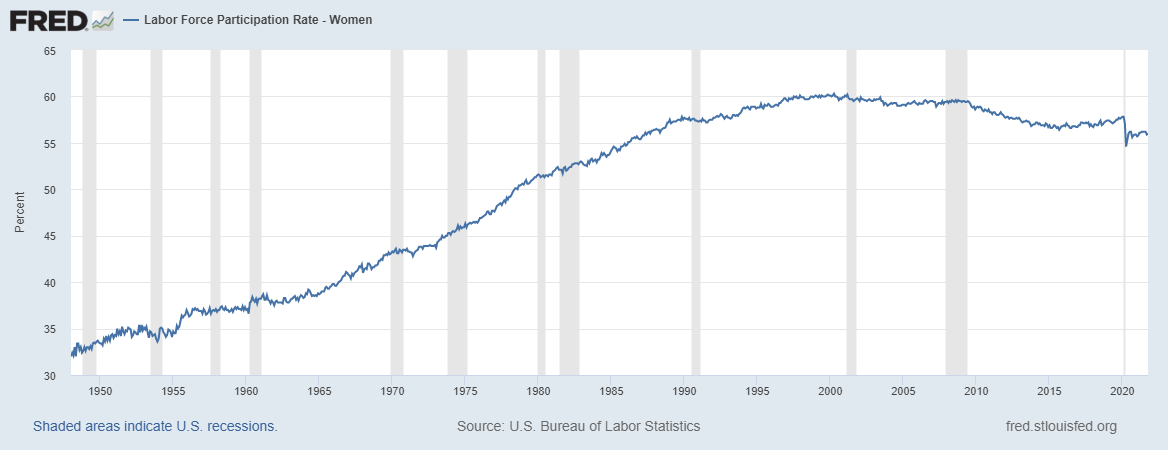
\includegraphics[scale=0.4]{fredgraph (3).png}
\caption{Percentage of Women in the Labor Force: 1948 - 2021}
\label{fig:Figure 1}
\end{figure}

\begin{figure}[h!]
\centering
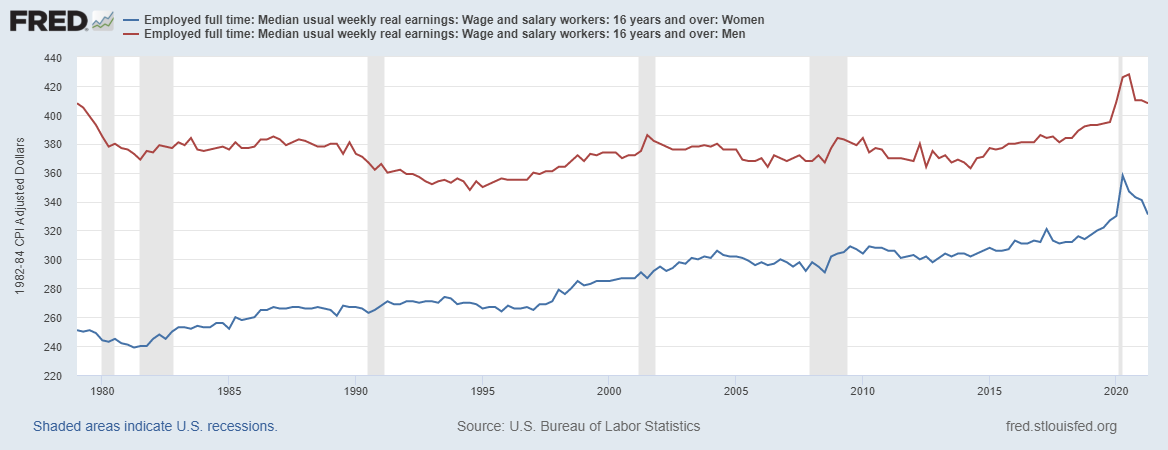
\includegraphics[scale=0.4]{fredgraph (2).png}
\caption{Comparison of Earnings Female (Blue) v. Male (Red): 1979-2021}
\label{fig:Figure 1}
\end{figure}

\newpage
\begin{table}[htp]
\centering % instead of \begin{center}
    \caption{Simple Regression Model}
    \vspace{7.5mm} % Adjust the height of the space between caption and tabular
\begin{tabular}[t]{lc}
\toprule
  & Model 1\\
\midrule
(Intercept) & 10.883\\
 & (0.002)\\
SEX & -0.513\\
 & (0.003)\\
\midrule
Num.Obs. & 654037\\
R2 & 0.059\\
R2 Adj. & 0.059\\
AIC & 1884290.1\\
BIC & 1884324.3\\
Log.Lik. & -942142.040\\
F & 41140.164\\
\bottomrule
\end{tabular}
\end{table}


\begin{table}[htp]
\centering % instead of \begin{center}
    \caption{Multi-Variable Regression Model}
    \vspace{7.5mm} % Adjust the height of the space between caption and tabular
\begin{tabular}[t]{lc}
\toprule
  & Model 1\\
\midrule
(Intercept) & 6.213\\
 & (0.018)\\
SEX & -0.479\\
 & (0.002)\\
RACENW & 0.010\\
 & (0.003)\\
EDUCYRS & 0.097\\
 & \vphantom{1} (0.001)\\
AGE & 0.129\\
 & (0.001)\\
(AGE\textasciicircum{}2) & -0.001\\
 & (0.000)\\
\midrule
Num.Obs. & 654014\\
R2 & 0.147\\
R2 Adj. & 0.147\\
AIC & 1820017.1\\
BIC & 1820096.8\\
Log.Lik. & -910001.546\\
F & 22572.563\\
\bottomrule
\end{tabular}
\end{table}



\newpage

\begin{table}[htp]
\centering % instead of \begin{center}
    \caption{Fixed Effects Model: Gender Wage Gap}
    \vspace{7.5mm} % Adjust the height of the space between caption and tabular
\begin{tabular}[t]{lcc}
\toprule
  & Gubernatorial Democrat Vote Share & Gubernatorial Republican Vote Share \\
\midrule
democrat & 0.001 & \\
 & (0.001) & \\
republican &  & -0.001\\
 &  & (0.001)\\
\midrule
Num.Obs. & 353 & 353\\
R2 & 0.458 & 0.457\\
R2 Adj. & 0.314 & 0.312\\
se\_type & HC2 & HC2\\
\bottomrule
\end{tabular}
\end{table}



\newpage

\end{document}



